%%%%%%%%%%%%%%%%%%%%%%%%%%%%%%%%%%%%%%%%%%%%%%%%%%%%%%%%%%%%%%%%%%%%%%%%%%%%% 
%
% This is a LaTeX file for an A3 poster.
%
%%%%%%%%%%%%%%%%%%%%%%%%%%%%%%%%%%%%%%%%%%%%%%%%%%%%%%%%%%%%%%%%%%%%%%%%%%%%% 

%%%%%%%%%%%%%%%%%%%%%%%%%%%%%%%%%%%%%%%%%%%%%%%%%%%%%%%%%%%%%%%%%%%%%%%%%%%%% 
%%%%%%%%%%%%%%%%%%%%%%%%%%%%%%%%%%%%%%%%%%%%%%%%%%%%%%%%%%%%%%%%%%%%%%%%%%%%%
%
% Asymptotic behavior of solutions to the generalized Becker-D�ring
% equations for general initial data.
%
% Poster for the HYKE-3 meeting in Rome, 13-15 April 2005.
% 
%%%%%%%%%%%%%%%%%%%%%%%%%%%%%%%%%%%%%%%%%%%%%%%%%%%%%%%%%%%%%%%%%%%%%%%%%%%%%
%%%%%%%%%%%%%%%%%%%%%%%%%%%%%%%%%%%%%%%%%%%%%%%%%%%%%%%%%%%%%%%%%%%%%%%%%%%%%
%,a1paper,landscape,
\documentclass{sciposter}
% To modify the size of the page:
%\usepackage[dvips,centering,left=0.5cm,top=0.5cm,right=0.5cm,bottom=0.5cm]{geometry}
\usepackage{lipsum}
\usepackage{epsfig}
\usepackage{amssymb}
\usepackage{url}

\usepackage{multirow} 
\usepackage{multicol}
\usepackage[latin1]{inputenc}
\usepackage{color}


\usepackage{amsmath, amsthm, amsfonts}
\usepackage{graphicx}           % Include figure files.
\usepackage{verbatim}
\usepackage{wrapfig}
\usepackage[dvipsnames]{xcolor}

% Colors
% -------
\definecolor{azulillo}{rgb}{0.8,0.85,1}
\definecolor{marronrp3}{rgb}{.9,.9,.7}
\definecolor{salmon}{rgb}{1,.9,.8}
\definecolor{rojo}{rgb}{.6,.1,0}

\pagestyle{empty}

\def\to{\rightarrow}

% Hyphenation
\hyphenation{coa-gu-la-tion frag-men-ta-tion}

% ===========================================================================

\title{}
\author{}
\date{}

\begin{document}
%\maketitle

\begin{center}
  \begin{minipage}{.19\linewidth}
    
\includegraphics[width=.7\linewidth]{logolatinr.jpg}
  \end{minipage}
  %&
  \begin{minipage}{.6\linewidth}
    \begin{center}
      \Huge \textbf{Paquete ZOIP de R para modelo de regresi\'{o}n mixto con datos proporcionales inflados con ceros y/o unos}
    \end{center}
  \end{minipage}
  %&
  \hspace{.03\linewidth}
  \begin{minipage}{0.16\linewidth}
    \begin{flushright}
     \textbf{ Juan Camilo D�az Zapata}\\
			twitter: @jkmilodiaz  github.com/jucdiaz/ZOIP \\
			\textbf{Freddy Hern�ndez Barajas}\\
			twitter: @fhernanb74 \\
      \textit{Escuela de Estad�stica}\\
		\textit{\textbf{Universidad Nacional de Colombia, Medell�n}}\\
    \end{flushright}
  \end{minipage}
\end{center}

\vspace{.1cm}

% ---------------------------------------------------------------------------

\setlength{\multicolsep}{1cm}
\begin{multicols}{2}

\noindent
\colorbox{SkyBlue}{
  \begin{minipage}[t]{.96\linewidth}
    \vspace{.05cm}
   \begin{center}
      \section*{\LARGE Introducci�n}
	\end{center}
Los modelos de regresi�n mixto para datos proporcionales inflados con ceros y/o unos, son �tiles para determinar el comportamiento de una variable proporcional a partir de variables consideradas como efectos fijos y aleatorios.\\

La integraci�n de los modelos estad�sticos en un paquete del sistema computacional \textit{R} permite que la utilizaci�n de los modelos estad�sticos a problemas aplicados sea de gran facilidad para la comunidad estad�stica. 
  \end{minipage}
}

\vspace{.2cm}
{\LARGE 
\begin{center}
\textbf{Estado del arte}
\end{center}
}

\begin{center}
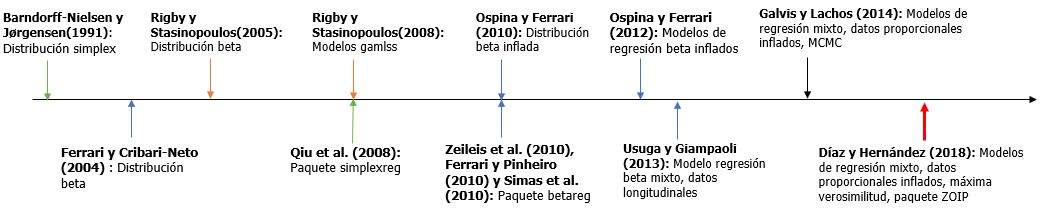
\includegraphics[width=1\linewidth]{Estado_Arte.jpg} 
\end{center}

{\LARGE
\begin{center}
\textbf{Distribuci�n ZOIP (Zeros Ones Inflated Proportional)}
\end{center}
}
Si la variable aleatoria $Y$ tiene distribuci�n ZOIP con par�metros $\mu$, $\sigma$, $p_0$ y $p_1$, se denotar� como $Y \sim$ ZOIP$(\mu,\sigma, p_0, p_1)$, la funci�n de densidad de probabilidad est� dada por:

\begin{equation*}
g(y;\mu,\sigma, p_{0}, p_{1})=
\begin{cases}
p_{0} & \text{si}\ y=0,\\
p_{1} & \text{si}\ y=1,\\
(1-p_{0}-p_{1})f(y;\mu,\sigma) & \text{si}\ y \in (0,1)
\end{cases}
 %\label{eq_Dist_ZOIP}
\end{equation*}

donde $p_{0} \geq 0$ y $p_{1} \geq 0$, adem\'{a}s $f(y;\mu,\sigma)$ representa alguna de las funciones de densidad de probabilidad para datos proporcionales

{\LARGE 
\begin{center}
\textbf{Modelo de regresi\'{o}n ZOIP con efectos mixtos}
\end{center}
}

Sea $y_{ij}$ la $j-$\'{e}sima medida del $i-$\'{e}simo grupo, una formulaci\'{o}n matem\'{a}tica para el modelo es la siguiente:

\begin{align}
\begin{split}
y_{ij}| \gamma_{1i},\gamma_{2i} & \overset{\text{ind}}{\sim} ZOIP(\mu_{ij},\sigma_{ij},p_{0ij}, p_{1ij}),\\
	h_1(\mu_{ij}) &= \mathbf{x}_{ij1}^{\top} \boldsymbol{\beta}_1+ \gamma_{1i},\\
	h_2(\sigma_{ij}) &= \mathbf{x}_{ij2}^{\top} \boldsymbol{\beta}_2+ \gamma_{2i},\\
	h_3(p_{0ij}) &= \mathbf{x}_{ij3}^{\top} \boldsymbol{\beta}_3,\\
	h_4(p_{1ij}) &= \mathbf{x}_{ij4}^{\top} \boldsymbol{\beta}_4,\\
	\gamma_{1i} & \overset{\text{i.i.d}}{\sim}  N(0,\lambda_1^2),\\
	\gamma_{2i} & \overset{\text{i.i.d}}{\sim}  N(0,\lambda_2^2),
\end{split}
\label{Mod_pmix}
\end{align}
con $i=1,2,\ldots, N$ y $j=1,2,\ldots, n_i$.

% ---------------------------------------------------------------------------
%\noindent
%\colorbox{marronrp3}{
  %\begin{minipage}[t]{.96\linewidth} 
\begin{center}
\LARGE{\textbf{Estimaci�n v�a m�xima verosimilitud y AGHQ}}
\end{center}
El vector de par\'{a}metros para el modelo \eqref{Mod_pmix} es $\boldsymbol{\theta}=(\boldsymbol{\beta_1}^{\top},\boldsymbol{\beta_2}^{\top},\boldsymbol{\beta_3}^{\top}, \boldsymbol{\beta_4}^{\top},\lambda_1,\lambda_2)^{\top}$ y de esa forma la funcion de log-verosimilitud $\ell(\boldsymbol{\theta})$ esta dado por:

\begin{equation*}
\ell(\boldsymbol{\theta})=\sum_{i=1}^{N}log \left[\int_{\mathbb{R}^2}\prod_{j=1}^{n_i}f_y(y_{ij}|\gamma_{1i},\gamma_{2i};\boldsymbol{\beta_1}, \boldsymbol{\beta_2}, \boldsymbol{\beta_3}, \boldsymbol{\beta_4})\cdot f(\gamma_{1i}|\lambda_1) f(\gamma_{2i}|\lambda_2) d\gamma_{1i}d\gamma_{2i}\right]
 %\label{func_ver_mix}
\end{equation*}

Para encontrar el punto m�ximo de la funci�n de log-verosimilitud anterior, es necesario rea\-li\-zar una aproximaci�n por medio de la cuadratura de Gauss-Hermite adaptativa con o sin \textit{pruning}

					 %\end{minipage}
					%}
				    \vspace{0.4cm}				
\noindent
\colorbox{SeaGreen}{
  \begin{minipage}[t]{.96\linewidth} 
\begin{center}
{\LARGE \textbf{Paquete ZOIP de R}}
\end{center}
			    \vspace{.02cm}
El paquete \textit{ZOIP} de \textit{R} es �til para ajustar distribuci�n ZOIP, modelos de regresi�n de efectos fijos y mixtos para datos proporcionales inflados con ceros y/o unos. Estas son las principales funciones: \\ %\medskip
\begin{center}
\texttt{dZOIP}  \hspace{.05cm}   \texttt{pZOIP} \hspace{.05cm} \texttt{qZOIP} \hspace{.05cm} \texttt{rZOIP} \hspace{.05cm} \texttt{RM.ZOIP} \hspace{.05cm} \texttt{RMM.ZOIP}
\end{center}

					 \end{minipage}
					}

\begin{center}

\includegraphics[width=0.3\linewidth]{Logo_ZOIP.jpg} 
\end{center}

%
%\begin{wrapfigure}{r}{0.5\textwidth}
 %\centering
		%
\includegraphics[scale=0.45]{Logo_ZOIP.jpg}
%\end{wrapfigure}

%\begin{verbatim}
%RM.ZOIP(formula.mu, formula.sigma = ~1, formula.p0 = ~1, 
        %formula.p1 = ~1, data, link = c("identity", "identity", 
        %"identity", "identity"), family = "R-S",
				%optimizer = "nlminb")
%\end{verbatim}

Ejemplo:

\begin{verbatim}
link <- c("logit", "logit", "identity", "logit")
mod<-RM.ZOIP(formula.mu = y_i ~ x1, formula.sigma = ~x1 + x2,
        formula.p0 = ~1, formula.p1 = ~x2, data = base, 
        link = link, family = "R-S")
				
summary(mod)
\end{verbatim}

%\begin{verbatim}
%RMM.ZOIP(formula.mu, formula.sigma = ~1, formula.p0 = ~1, 
         %formula.p1 = ~1, data, formula.random,
				 %link = c("identity","identity", "identity", "identity"),
				 %family = "R-S", optimizer = "nlminb",
				 %n.points = 11, pruning = TRUE)
%\end{verbatim}

\begin{verbatim}
link <- c("logit", "logit", "identity", "identity")
mod<-RMM.ZOIP(formula.mu = Y ~ log(Days), formula.sigma = ~log(Days), 
         formula.p0 = ~1, formula.p1 = ~1, data = base, 
         formula.random = ~1 | subject, link = link, family = "R-S")
				
summary(mod)
\end{verbatim}
\vspace{8cm}

{\LARGE
\begin{center}
\textbf{Aplicaci�n modelo de regresi�n ZOIP mixto}
\end{center}
}

Se plante\'{o} un modelo de regresi\'{o}n ZOIP-beta con intercepto aleatorio en el par\'{a}metro de la media y la varianza, dado por la variable \textsl{ciudad} y un efecto fijo en la media y la varianza dado por la variable \textsl{total mora}, para la variable respuesta \textbf{porcentaje de utilizaci�n de una tarjeta de cr�dito (tdc)}.
\begin{equation*}
\begin{split}
y_{ij}| \gamma_{1i},\gamma_{2i} &\overset{\text{ind}}{\sim} ZOIP(\mu_{ij},\sigma_{ij},p_0, p_1),\\
h_1(\mu_{ij})&=\beta_{10}+\gamma_{1i}+\beta_{11} x_{1ij},\\
h_2(\sigma_{ij})&=\beta_{20}+\gamma_{2i}+\beta_{21} x_{1ij},\\
h_3(p_{0})&=\beta_{30},\\
h_4(p_{1})&=\beta_{40},
\end{split}
%\label{A_eq_reg_mix}
\end{equation*}

con $\gamma_{1i} \sim N(0, \lambda_1^2)$ y $\gamma_{2i} \sim N(0, \lambda_2^2)$.\\

$y_{ij}$ es el porcentaje de utilizaci\'{o}n de la $j$-\'{e}sima tdc perteneciente a la $i$-\'{e}sima ciudad, $i=1,2,\ldots, 10$ y $j=1,2,\ldots, 15$.\\

$x_{1ij}$: es el valor del tiempo en mora en meses de la $j$-\'{e}sima tdc asociada a la $i$-\'{e}sima ciudad.\\

El modelo propuesto se puede reescribir con los par\'{a}metros estimados por medio del paquete  \texttt{ZOIP} y la funci�n  \texttt{RMM.ZOIP}, as\'{\i}:

\begin{equation}
\begin{split}
y_{ij}| \gamma_{1i},\gamma_{2i} & \overset{\text{ind}}{\sim} ZOIP(\mu_{ij},\sigma_{ij},p_0, p_1),\\
h_1(\mu_{ij})&=-1.13+\gamma_{1i}+0.33 x_{1ij},\\
h_2(\sigma_{ij})&=0.33+\gamma_{2i}+0.14 x_{1ij},\\
h_3(p_{0})&=0.23,\\
h_4(p_{1})&=0.07,
\end{split}
\label{A_eq_reg_mix2}
\end{equation}

donde $\gamma_{1i} \sim N(0, 0.51^2)$ y $\gamma_{2i} \sim N(0, 0.40^2)$.

\vspace{0.4cm}

\noindent
\colorbox{SeaGreen}{
  \begin{minipage}[t]{.96\linewidth} 
\begin{center}
{\LARGE \textbf{Estudio de simulaci�n: Modelo regresi�n ZOIP mixto}}
\end{center}
			    \vspace{.02cm}
					
El modelo de regresi�n ZOIP mixto en el cual se basa el estudio de simulaci�n esta dado por \eqref{A_eq_reg_mix2} y el esquema de simulacion es:
					 \end{minipage}
					}

\begin{center}
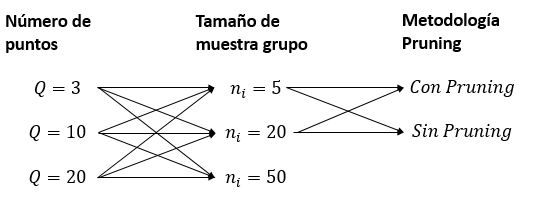
\includegraphics[width=0.7\linewidth]{Esc_sim_mix.jpg}
		\caption{Esquema de simulaci�n.}
\end{center}

En el estudio de simulaci�n se plantearon 18 escenarios de simulaci\'{o}n y se realizaron 1000 r\'{e}plicas en cada escenario, dando como resultado:

%%%%%%%%%%%%%%%%%%%%%%%%%%%%

\begin{table}[!hbt]
{\normalsize
\begin{center}
\begin{tabular}{|c|c|c|c|c|c|c|c|}\hline
& & \multicolumn{3}{|c|}{Con \textit{pruning}} & \multicolumn{3}{|c|}{Sin \textit{pruning}} \\ \hline
Par\'{a}metro &$\beta$'s & $n_i=5$ & $n_i=20$ & $n_i=50$ & $n_i=5$ & $n_i=20$ & $n_i=50$ \\ \hline \hline
\multirow{3}{*}{$\mu$} & $\beta_{10}=-1.13$ & -1.137	&-1.110	&-1.076	&-1.128	&-1.120	&-1.080 \\ 
& $\beta_{11}=0.33$ & 0.321	&0.327	&0.326	&0.331	&0.330	&0.327 \\
& $\lambda_1=0.51$ & 0.879	&0.576	&0.507	&0.882	&0.568	&0.498 \\ \hline
\multirow{3}{*}{$\sigma$} & $\beta_{20}=0.33$ & 0.445	&0.380	&0.336	&0.452	&0.377	&0.345 \\ 
& $\beta_{21}=0.14$ & 0.072	&0.118	&0.132	&0.066	&0.121	&0.133\\
& $\lambda_2=0.4$ & 0.728	&0.450	&0.396	&0.727	&0.456	&0.398\\ \hline
$p_0$& $\beta_{30}=0.23$ &0.220	&0.230	&0.230	&0.220	&0.230	&0.230 \\ \hline
$p_1$& $\beta_{40}=0.07$ &0.060	&0.070	&0.070	&0.060	&0.070	&0.072 \\ \hline
Med tiempo(Seg)& &115.72	&130.85	&140.58	&61.69	&163.36	&218.68 \\ \hline
Med num. iter& &22	&30	&34	&22	&30	&34 \\ \hline
\end{tabular}
\caption{Resultados del estudio de simulaci�n}
%\caption{Mediana de los par\'{a}metros estimados en el modelo ZOIP mixto para tres tama\~{n}os de muestra y con la estrategia de ``con y sin \textit{pruning}'' y para todos los valores de $Q$.}
\label{T_Sim_mix_ni}
\end{center}
}
\end{table}

%%%%%%%%%%%%%%%%%%%%%%%%%%%%



{\LARGE
\begin{center}
\textbf{Conclusiones}
\end{center}
}

\begin{enumerate}
	\item El paquete \textit{ZOIP} se implementan diferentes funciones, con el objetivo de que sean utilizados los modelos de regresi�n ZOIP por un usuario. Dicho paquete muestra convergencia de sus funciones desarrollados, por medio de los estudios de simulaci�n.
	\item Los factores que m\'{a}s influyen sobre la estimaci\'{o}n es el tama\~{n}o de muestra de cada uno de los grupos, es decir $n_i$, ya que este factor hace que el error relativo de la estimaci\'{o}n de todos los par\'{a}metros se vea reducido considerablemente cuando se aumenta.
	\item El hecho de utilizar la metodolog\'{\i}a \textit{pruning} hace que los valores de las estimaciones de los par\'{a}metros del modelo no cambien, pero s\'{\i} que el tiempo de ejecuci\'{o}n se vea reducido en un 50\%.
	\end{enumerate}


% ---------------------------------------------------------------------------
%,Jorgensen1,R,Stasinopoulos1,Qiu1,Usuga1,Ospina2
\small
\nocite{Ferrari2,Stasinopoulos2,Barndorff1,Galvis1,Ospina1,Zeileis1}
  
  \bibliographystyle{abbrv}
  \bibliography{symposium}

\end{multicols}

\end{document}